\newpage

\subsection{QuizziPedia::Front-End::ModelViews}
\subsubsection{Informazioni generali}
\label{QuizziPedia::Front-End::ModelViews}
\begin{figure}
	\centering
	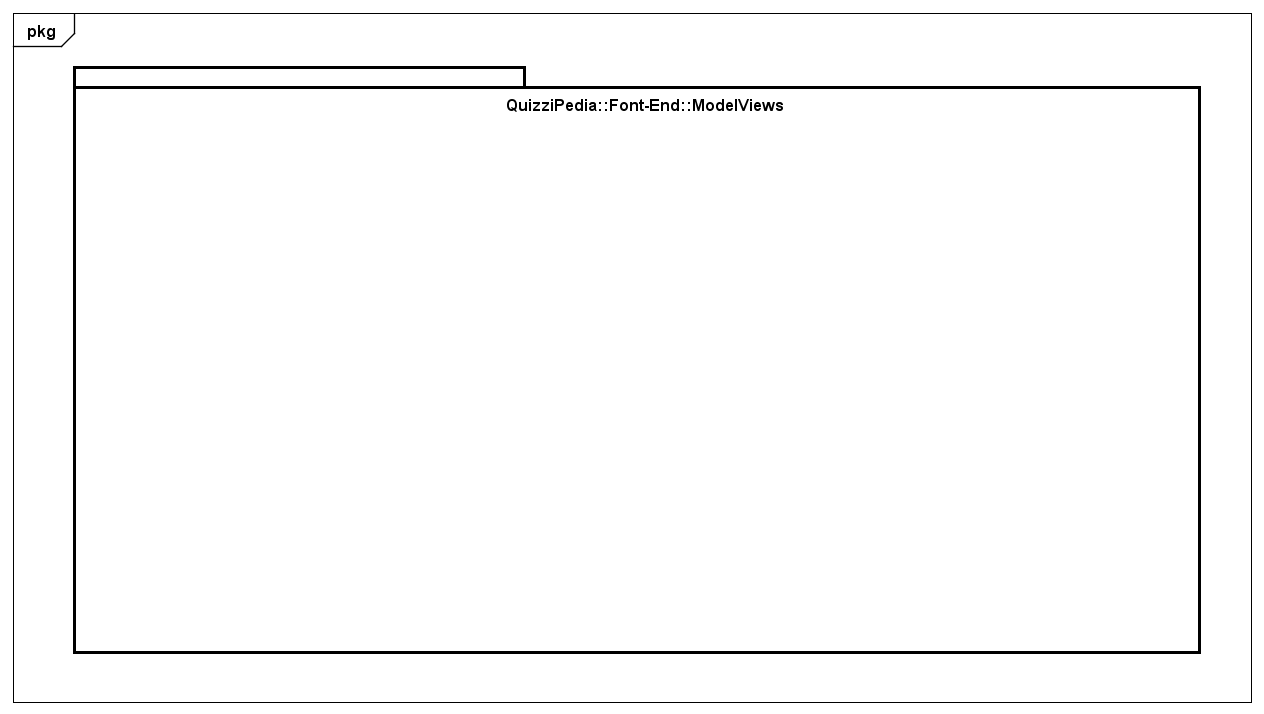
\includegraphics[scale=0.45]{UML/Package/QuizziPedia_Front-End_ModelViews.png}
	\caption{QuizziPedia::Front-End::ModelViews}
\end{figure}
\begin{itemize}
	\item \textbf{Descrizione}: package contenente le classi che saranno presenti nella variabile d'ambiente \texttt{\$scope} di \textit{Angular.js\ped{G}} che permettono il \textit{Two-Way Data-Binding\ped{G}} tra le views e i controllers;
	\item \textbf{Padre}: \texttt{Front-End};
	\item \textbf{Interazione con altri componenti}:
	\begin{itemize}
		\item \texttt{Controllers}: package contenente i controllers front-end dell'applicazione;
		\item \texttt{Directives}: package contenente le directives front-end dell'applicazione;
		\item \texttt{View}: package contenente le views front-end dell'applicazione;
		\item \texttt{Templates}: package contenente i templates necessari per la creazione dinamica delle viste per le domande.
	\end{itemize}
\end{itemize}
\subsubsection{Classi}
	
	\paragraph{QuizziPedia::Front-End::ModelViews::ClickableAreaQuestionsModelView}
\begin{figure} [ht]
	\centering
	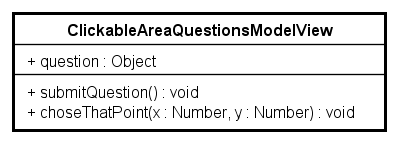
\includegraphics[scale=0.80]{UML/Classi/Front-End/QuizziPedia_Front-end_ModelView_ClickableAreaQuestionsModelView.png}
	\caption{QuizziPedia::Front-End::ModelViews::ClickableAreaQuestionsModelView}
\end{figure} \FloatBarrier
\begin{itemize}
	\item \textbf{Descrizione}: classe di tipo modelview la cui istanziazione è contenuta all'interno della variabile di ambiente \$scope di \textit{Angular.js\ped{G}}. All'interno di essa sono presenti le variabili e i metodi necessari per il \textit{Two-Way Data-Binding\ped{G}} tra la view \texttt{ClickableAreaQuestionsView} e il controller \texttt{ClickableAreaQuestionsController}; 
	\item \textbf{Utilizzo}: viene utilizzata per effettuare il \textit{Two-Way Data-Binding\ped{G}} tra la view \texttt{ClickableAreaQuestionsView} e il controller \texttt{ClickableAreaQuestionsController} rendendo disponibili variabili e metodi;
	\item \textbf{Relazioni con altre classi}:
	\begin{itemize}
		\item \textit{IN} \texttt{ClickableAreaQuestionsView}: view contenente i campi e le direttive per creare una domanda ad area cliccabile; 
		\item \textit{IN} \texttt{ClickableAreaQuestionsController}: questa classe permette di gestire la creazione e la modifica di una domanda ad area cliccabile;
	\end{itemize}
	\item \textbf{Attributi}:
	\begin{itemize}
			\item \texttt{+ question: Object} \\ Oggetto contenente gli attributi per la creazione della domanda:
			\begin{itemize}
				\item \texttt{url: String}: attributo di tipo \texttt{String} che contiene l'\textit{URL\ped{G}} associato all'immagine;
				\item \texttt{answer: Array}: array contenente oggetti che rappresentano le risposte. Ogni oggetto risposta contiene:
				\begin{itemize}
					\item \texttt{x: Number}: attributo di tipo \texttt{Number} che rappresenta la posizione della risposta nell'asse delle ascisse all'interno dell'immagine;
					\item \texttt{y: Number}: attributo di tipo \texttt{Number} che rappresenta la posizione della risposta nell'asse delle ordinate all'interno dell'immagine.
				\end{itemize}
	\end{itemize}
	\item \textbf{Metodi}:
	\begin{itemize}
			\item \texttt{+} \texttt{submitQuestion(): void}\\ 
			Metodo che gestisce l’evento click sul pulsante di conferma sulla domanda. Raccoglie i dati dal modelview e li manda al server attraverso \texttt{QuestionService}. Poi verrà effettuato il redirect alla pagina di gestione delle domande oppure al questionario che si stava creando; 
			\item \texttt{+} \texttt{choseThatPoint(x: Number, y: Number): void}\\
			Metodo che gestisce l’evento click su un punto dell'immagine. Una volta selezionato esso verrà inserito nell'array di punti; \\
			\textbf{Parametri}:
			\begin{itemize}
				\item \texttt{x: Number} \\
				Parametro contenente la coordinata x del punto;
				\item \texttt{y: Number} \\ 
				Parametro contenente la coordinata y del punto;
			\end{itemize}
	\end{itemize}
\end{itemize}
\end{itemize}


	\paragraph{QuizziPedia::Front-End::ModelViews::ConnectionQuestionsModelView}
\begin{figure} [ht]
	\centering
	%\includegraphics[scale=0.80]{UML/Classi/Front-End/QuizziPedia_Front-end_Views_ConnectionQuestionsModelView.png}
	\caption{QuizziPedia::Front-End::ModelViews::ConnectionQuestionsModelView}
\end{figure} \FloatBarrier
\begin{itemize}
	\item \textbf{Descrizione}: classe di tipo modelview la cui istanziazione è contenuta all'interno della variabile di ambiente \$scope di \textit{Angular.js\ped{G}}. All'interno di essa sono presenti le variabili e i metodi necessari per il \textit{Two-Way Data-Binding\ped{G}} tra la view \texttt{ConnectionQuestionsView} e il controller \texttt{ConnectionQuestionsController}; 
	\item \textbf{Utilizzo}: viene utilizzata per effettuare il \textit{Two-Way Data-Binding\ped{G}} tra la view \texttt{ConnectionQuestionsView} e il controller \texttt{ConnectionQuestionsController} rendendo disponibili variabili e metodi;
	\item \textbf{Relazioni con altre classi}:
	\begin{itemize}
		\item \textit{IN} \texttt{ConnectionQuestionsView}: view contenente i campi e le direttive per creare una domanda a collegamento; 
		\item \textit{IN} \texttt{ConnectionQuestionsController}: questa classe permette di gestire la creazione e la modifica di una domanda a collegamento;
	\end{itemize}
	\item \textbf{Attributi}:
	\begin{itemize}
		\item \texttt{+ question: Object} \\ Oggetto contenente gli attributi per la creazione della domanda:
		\begin{itemize}
			\item \texttt{answer}: array contenente oggetti che rappresentano le risposte. Ogni oggetto risposta contiene:
			\begin{enumerate}
				\item \texttt{text1}: di tipo \texttt{String}, rappresenta il primo elemento testuale che sarà collegato ad un secondo elemento (testuale o immagine);
				\item \texttt{text2}:  di tipo \texttt{String}, rappresenta il secondo elemento testuale che sarà collegato al primo elemento (testuale o immagine);
				\item \texttt{url1}: di tipo \texttt{String}, rappresenta il primo elemento immagine che sarà collegato con il secondo elemento (testuale o immagine);
				\item \texttt{url2}: di tipo \texttt{String}, rappresenta il secondo elemento immagine che sarà collegato con il primo elemento (testuale o immagine).
			\end{enumerate}
		\end{itemize}
		\item \texttt{+ keyword: String} \\ Attributo contenente la keyword associata alla domanda/questionario;		
	\end{itemize}
	\item \textbf{Metodi}:
	\begin{itemize}
		\item \texttt{+} \texttt{submitQuestion(): void}\\ 
		Metodo che gestisce l’evento click sul pulsante di conferma sulla domanda. Raccoglie i dati dal modelview e li manda al server attraverso \texttt{QuestionService}. Poi verrà effettuato il redirect alla pagina di gestione delle domande oppure al questionario che si stava creando;  
	\end{itemize}
\end{itemize}


	\paragraph[QuizziPedia::Front-End::ModelViews\\::CreateQuestionnaireModelView]{QuizziPedia::Front-End::ModelViews::CreateQuestionnaireModelView}
	
	\label{QuizziPedia::Front-End::ModelViews::CreateQuestionnaireModelView}
	
	\begin{figure}[ht]
		\centering
		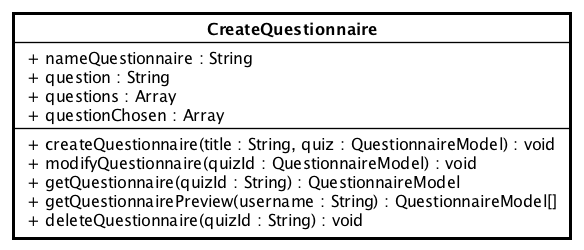
\includegraphics[scale=0.5,keepaspectratio]{UML/Classi/Front-End/QuizziPedia_Front-end_ModelView_CreateQuestionnaireModelView.png}
		\caption{QuizziPedia::Front-End::ModelViews::CreateQuestionnaireModelView}
	\end{figure} \FloatBarrier
	
	\begin{itemize}
		\item \textbf{Descrizione}: classe di tipo modelview la cui istanziazione è contenuta all'interno della variabile di ambiente \texttt{\$scope} di \textit{Angular\ped{G}}. All'interno di essa sono presenti le variabili e i metodi necessari per il \textit{Two-Way Data-Binding\ped{G}} tra la \textit{view\ped{G}} \texttt{CreateQuestionnaireView} e il \textit{controller\ped{G}} \texttt{CreateQuestionnaireController};
		\item \textbf{Utilizzo}: viene utilizzata per effettuare il \textit{Two-Way Data-Binding\ped{G}} tra la \textit{view\ped{G}}\\ \texttt{CreateQuestionnaireView} e il \textit{controller\ped{G}} \texttt{CreateQuestionnaireController} rendendo disponibili variabili e metodi;
		\item \textbf{Relazioni con altre classi}: 
		\begin{itemize}
			\item \textbf{OUT \texttt{CreateQuestionnaireView}}: \textit{view\ped{G}} per la creazione del questionario; 
			\item \textbf{OUT \texttt{CreateQuestionnaireController}}: questa classe permette di gestire la creazione di un questionario.
		\end{itemize}
		\item \textbf{Attributi}: 
		\begin{itemize}
			\item \texttt{+ nameQuestionnaire: String}: \\ Attributo che specifica il nome del questionario creato;
			\item \texttt{+ question: String} \\ Attributo che conterrà la stringa per la ricerca della domanda;
			\item \texttt{+ questions: Array} \\ \texttt{array} contenente le domande trovate durante la ricerca;
			\item \texttt{+ questionsChosen: Array} \\ \texttt{array} contenente le domande inserite nel questionario.
		\end{itemize}
		\item \textbf{Metodi}: 
		\begin{itemize}
			\item \texttt{+ createQuestionnaire(title: String, \\quiz: QuestionnaireModel) : void} \\Metodo che permette di inserire un questionario nel database tramite richiesta al service. \\
			\textbf{Parametri}:
			\begin{itemize}
				\item \texttt{title: String} \\ Parametro che indica il nome del questionario;
				\item \texttt{quiz: QuestionnaireModel} \\ Parametro che racchiude tutti i dati di un questionario.
			\end{itemize}
			\item \texttt{+ modifyQuestionnaire(quizId: QuestionnaireModel): void} \\ Metodo che serve per modificare un questionario. \\
			\textbf{Parametri}:
			\begin{itemize}
				\item \texttt{quiz: QuestionnaireModel}\\
				Parametro che rappresenta l'oggetto questionario.
			\end{itemize}
			\item \texttt{+ getQuestionnaire(quizId: String): QuestionnaireModel} \\Metodo che serve per ottenere un questionario tramite l'id in modo da poterlo modificare. \\
			\textbf{Parametri}:
			\begin{itemize}
				\item \texttt{quizId: String}\\
				Parametro che rappresenta l'id del questionario da richiedere.
			\end{itemize}
			\item \texttt{+ getQuestionnairePreview(username: String): Array<QuestionnaireModel>} \\ Metodo che serve per ottenere la lista di tutti i questionari di un utente. \\
			\textbf{Parametri}:
			\begin{itemize}
				\item \texttt{username: String}\\
				Parametro che indica l'utente del quale vogliamo caricare tutti i questionari.
			\end{itemize}
			\item \texttt{+ deleteQuestionnaire(quizId: String): void} \\ 
			Metodo che elimina un questionario. \\
			\textbf{Parametri}:
			\begin{itemize}
				\item \texttt{quizId: String}\\
				Identificativo del questionario da eliminare.
			\end{itemize}
			
			\item \texttt{- getQuestions(): Array<String>} \\
			Metodo che permette di ottenere la lista di tutte le domande.
			
			\item \texttt{- getQuestion(questionId: String): QuestionItemModel} \\
			Metodo che ritorna l'intera domanda selezionata. \\
			\textbf{Parametri}:
			\begin{itemize}
				\item \texttt{questionId: String}\\
				Parametro che indica l'identificativo univoco di una domanda.
			\end{itemize}
			\item \texttt{- addQuestion(questionId: String) : void} \\
			Metodo che permette di inserire una domanda nel questionario. \\
			\textbf{Parametri}:
			\begin{itemize}
				\item \texttt{questionId: String}\\
				Parametro che indica l'identificativo univoco di una domanda.
			\end{itemize}
		\end{itemize}
	\end{itemize}
	
	
	\paragraph{QuizziPedia::Front-End::ModelViews::EditorQMLModelView}
\begin{figure} [ht]
	\centering
	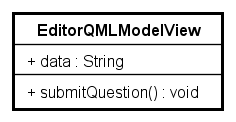
\includegraphics[scale=0.80]{UML/Classi/Front-End/QuizziPedia_Front-end_Views_EditorQMLModelView.png}
	\caption{QuizziPedia::Front-End::ModelViews::EditorQMLModelView}
\end{figure} \FloatBarrier
\begin{itemize}
	\item \textbf{Descrizione}: classe di tipo modelview la cui istanziazione è contenuta all'interno della variabile di ambiente \$scope di \textit{Angular.js\ped{G}}. All'interno di essa sono presenti le variabili e i metodi necessari per il \textit{Two-Way Data-Binding\ped{G}} tra la view \texttt{EditorQMLView} e il controller \texttt{EditorQMLController}; 
	\item \textbf{Utilizzo}: viene utilizzata per effettuare il \textit{Two-Way Data-Binding\ped{G}} tra la view \texttt{EditorQMLView} e il controller \texttt{EditorQMLController} rendendo disponibili variabili e metodi;
	\item \textbf{Relazioni con altre classi}:
	\begin{itemize}
		\item \textit{IN} \texttt{EditorQMLView}: view contenente l'editor QML per la creazione di domande personalizzate; 
		\item \textit{IN} \texttt{EditorQMLController}: questa classe permette di gestire la creazione e la modifica di domande create tramite editor QML;
	\end{itemize}
	\item \textbf{Attributi}:
	\begin{itemize}
		\item \texttt{+ data: String} \\ Stringa contenente il testo inserito dall'utente nell'apposito \textit{Editor\ped{G}}.
	\end{itemize}
	\item \textbf{Metodi}:
	\begin{itemize}
		\item \texttt{+} \texttt{submitQuestion(): void}\\ 
		Metodo che gestisce l’evento click sul pulsante di conferma sulla domanda. Raccoglie i dati dal modelview, li converte attraverso il parser QML, e li manda al server attraverso \texttt{QuestionService}. Poi verrà effettuato il redirect alla pagina di gestione delle domande oppure al questionario che si stava creando;
	\end{itemize}
\end{itemize}
		\paragraph{QuizziPedia::Front-End::ModelViews::FillingQuestionnaireModelView}
	
	\label{QuizziPedia::Front-End::ModelViews::FillingQuestionnaireModelView}
	
	\begin{figure}[ht]
		\centering
		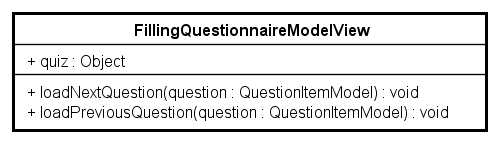
\includegraphics[scale=0.8,keepaspectratio]{UML/Classi/Front-End/QuizziPedia_Front-end_ModelView_FillingQuestionnaireModelView.png}
		\caption{QuizziPedia::Front-End::ModelViews::FillingQuestionnaireModelView}
	\end{figure} \FloatBarrier
	
	\begin{itemize}
		\item \textbf{Descrizione}: classe di tipo modelview la cui istanziazione è contenuta all'interno della variabile di ambiente \texttt{\$scope} di \textit{Angular\ped{G}}. All'interno di essa sono presenti le variabili e i metodi necessari per il \textit{Two-Way Data-Binding\ped{G}} tra la \textit{view\ped{G}} \texttt{FillingQuestionnaireView} e il \textit{controller\ped{G}} \texttt{FillingQuestionnaireController};
		\item \textbf{Utilizzo}: viene utilizzata per effettuare il \textit{Two-Way Data-Binding\ped{G}} tra la \textit{view\ped{G}}\\ \texttt{FillingQuestionnaireView} e il \textit{controller\ped{G}} \texttt{FillingQuestionnaireController} rendendo disponibili variabili e metodi;
		\item \textbf{Relazioni con altre classi}: 
		\begin{itemize}
			\item \textbf{OUT \texttt{FillingQuestionnaireView}}: \textit{view\ped{G}} principale per la compilazione del questionario. Conterrà i vari templates di ogni domanda appartenente al questionario; 
			\item \textbf{OUT \texttt{FillingQuestionnaireController}}: questa classe permette di gestire la compilazione del questionario.
		\end{itemize}
		\item \textbf{Attributi}: 
		\begin{itemize}
			\item \texttt{+ quiz: Object} \\ Oggetto contenente al suo interno i seguenti campi:
			\begin{itemize}
				\item \texttt{+ title: String} \\ Attributo che rappresenta il titolo del questionario;
				\item \texttt{+ argument: String} \\ Attributo che rappresenta l'argomento del questionario;
				\item \texttt{+ keywords: Array[String]} \\ \texttt{array} di stringhe che contiene le parole chiave del questionario;
				\item \texttt{+ questionNumber: String} \\ Attributo che rappresenta il numero progressivo della domanda attuale;
				\item \texttt{+ numberOfQuestions: String} \\ Attributo che rappresenta il numero di domande.
			\end{itemize}	
		\end{itemize}
		\item \textbf{Metodi}: 
		\begin{itemize}
			\item \texttt{+ loadNextQuestion(question: QuestionItemModel): void}\\
			Metodo che invoca l'evento per visualizzare la domanda successiva del quiz tramite \texttt{QuestionController}. \\
			\textbf{Parametri}:
			\begin{itemize}
				\item \texttt{question: QuestionItemModel} \\
				Parametro contenente un riferimento all'oggetto di tipo \texttt{QuestionItemModel}.
			\end{itemize}
			\item \texttt{+ loadPreviousQuestion(question: QuestionItemModel): void} \\
			Metodo che invoca l'evento per visualizzare la domanda precedente del quiz tramite \texttt{QuestionController}. \\
			\textbf{Parametri}:
			\begin{itemize}
				\item \texttt{question: QuestionItemModel} \\
				Parametro contenente un riferimento all'oggetto di tipo \texttt{QuestionItemModel}.
			\end{itemize}
			\item \texttt{+ startQuiz(): void} \\
			Metodo che gestisce l'evento per iniziare il questionario. 
		\end{itemize}
	\end{itemize}
	
	
	\paragraph{QuizziPedia::Front-End::ModelViews::FillingQuestionsModelView}
\begin{figure} [ht]
	\centering
	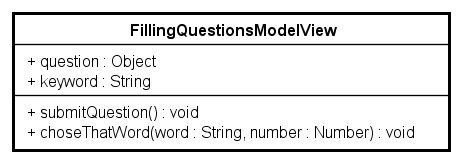
\includegraphics[scale=0.80]{UML/Classi/Front-End/QuizziPedia_Front-end_ModelView_FillingQuestionsModelView.png}
	\caption{QuizziPedia::Front-End::ModelViews::FillingQuestionsModelView}
\end{figure} \FloatBarrier
\begin{itemize}
	\item \textbf{Descrizione}: classe di tipo modelview la cui istanziazione è contenuta all'interno della variabile di ambiente \texttt{\$scope} di \textit{Angular\ped{G}}. All'interno di essa sono presenti le variabili e i metodi necessari per il \textit{Two-Way Data-Binding\ped{G}} tra la \textit{view\ped{G}} \texttt{FillingQuestionsView} e il \textit{controller\ped{G}} \texttt{FillingQuestionsController}; 
	\item \textbf{Utilizzo}: viene utilizzata per effettuare il \textit{Two-Way Data-Binding\ped{G}} tra la \textit{view\ped{G}}\\ \texttt{FillingQuestionsView} e il \textit{controller\ped{G}} \texttt{FillingQuestionsController} rendendo disponibili variabili e metodi;
	\item \textbf{Relazioni con altre classi}:
	\begin{itemize}
		\item \textbf{IN \texttt{FillingQuestionsView}}: \textit{view\ped{G}} contenente i campi e le direttive per creare una domanda a riempimento testo; 
		\item \textbf{IN \texttt{FillingQuestionsController}}: questa classe permette di gestire la creazione e la modifica di una domanda a riempimento di spazi.
	\end{itemize}
	\item \textbf{Attributi}:
	\begin{itemize}
		\item \texttt{+ question: Object} \\ Oggetto contenente gli attributi per la creazione della domanda:
		\begin{itemize}
			\item \texttt{answer: Array}: \texttt{array} contenente oggetti che rappresentano le risposte. Ogni oggetto risposta contiene:
			\begin{enumerate}
				\item \texttt{wordNumber: Number}: attributo di tipo \texttt{Number} che indica la parola nel testo che andrà inserita in fase di compilazione.
			\end{enumerate}
		\end{itemize}
		\item \texttt{+ keyword: String} \\ Attributo contenente la keyword associata alla domanda/questionario.
	\end{itemize}
	\item \textbf{Metodi}:
	\begin{itemize}
			\item \texttt{+ submitQuestion(): void}\\ 
			Metodo che gestisce l’evento click sul pulsante di conferma sulla domanda. Raccoglie i dati dal modelview e li manda al server attraverso \texttt{QuestionService}. Poi verrà effettuato il redirect alla pagina di gestione delle domande oppure al questionario che si stava creando; 
			\item \texttt{+ choseThatWord(word: String, number: Number): void}\\
			Metodo che gestisce l’evento click su una parola del testo. Una volta selezionata essa verrà inserita nell'array che conterrà le parole che dovranno essere nascoste quando l'esercizio sarà proposto. \\
			\textbf{Parametri}:
			\begin{itemize}
				\item \texttt{word: String} \\
				Parametro contenente la parola scelta da nascondere;
				\item \texttt{number: Number} \\ 
				Parametro che si riferisce al numero della parola scelta da nascondere.
			\end{itemize}
	\end{itemize}
\end{itemize}


	\paragraph{QuizziPedia::Front-End::ModelViews::HomeModelView}
	
	\label{QuizziPedia::Front-End::ModelViews::HomeModelView}
	
	\begin{figure}[ht]
		\centering
		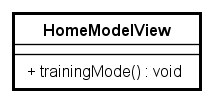
\includegraphics[scale=0.80,keepaspectratio]{UML/Classi/Front-End/QuizziPedia_Front-end_ModelView_HomeModelView.png}
		\caption{QuizziPedia::Front-End::ModelViews::HomeModelView}
	\end{figure} \FloatBarrier
	
	\begin{itemize}
		\item \textbf{Descrizione}: classe di tipo modelview la cui istanziazione è contenuta all'interno della variabile di ambiente \texttt{\$scope} di \textit{Angular\ped{G}}. All'interno di essa sono presenti le variabili e i metodi necessari per il \textit{Two-Way Data-Binding\ped{G}} tra la \textit{view\ped{G}} \texttt{HomeView} e il \textit{controller\ped{G}} \texttt{HomeController};
		\item \textbf{Utilizzo}: viene utilizzata per effettuare il \textit{Two-Way Data-Binding\ped{G}} tra la \textit{view\ped{G}} \texttt{HomeView} e il \textit{controller\ped{G}} \texttt{HomeController} rendendo disponibili variabili e metodi;
		\item \textbf{Relazioni con altre classi}: 
		\begin{itemize}
			\item \textbf{OUT \texttt{HomeView}}: \textit{view\ped{G}} contenente la direttiva per barra di ricerca degli utenti e questionari e il bottone che porterà l'utente nella modalità allenamento; 
			\item \textbf{OUT \texttt{HomeController}}: questa classe permette di gestire la home page;
		\end{itemize}
		\item \textbf{Metodi}: 
		\begin{itemize}
			\item \texttt{+ trainingMode(): void} \\
			Metodo che gestisce l’evento click sul pulsante di allenamento. Effettua il redirect alla pagina di allenamento.
		\end{itemize}
	\end{itemize}
	
	
	\paragraph{QuizziPedia::Front-End::ModelViews::ImagesSortingQuestionsModelView}
\begin{figure} [ht]
	\centering
	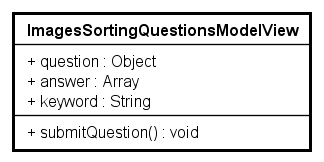
\includegraphics[scale=0.80]{UML/Classi/Front-End/QuizziPedia_Front-end_ModelView_ImagesSortingQuestionsModelView.png}
	\caption{QuizziPedia::Front-End::ModelViews::ImagesSortingQuestionsModelView}
\end{figure} \FloatBarrier
\begin{itemize}
	\item \textbf{Descrizione}: classe di tipo modelview la cui istanziazione è contenuta all'interno della variabile di ambiente \texttt{\$scope} di \textit{Angular\ped{G}}. All'interno di essa sono presenti le variabili e i metodi necessari per il \textit{Two-Way Data-Binding\ped{G}} tra la \textit{view\ped{G}} \texttt{ImagesSortingQuestionsView} e il \textit{controller\ped{G}} \texttt{ImagesSortingQuestionsController}; 
	\item \textbf{Utilizzo}: viene utilizzata per effettuare il \textit{Two-Way Data-Binding\ped{G}} tra la \textit{view\ped{G}}\\ \texttt{ImagesSortingQuestionsView} e il \textit{controller\ped{G}} \texttt{ImagesSortingQuestionsController} rendendo disponibili variabili e metodi;
	\item \textbf{Relazioni con altre classi}:
	\begin{itemize}
		\item \textbf{IN \texttt{ImagesSortingQuestionsView}}: \textit{view\ped{G}} contenente i campi e le direttive per creare una domanda a ordinamento immagini; 
		\item \textbf{IN \texttt{ImagesSortingQuestionsController}}: questa classe permette di gestire la creazione e la modifica di una domanda a ordinamento immagini.
	\end{itemize}
	\item \textbf{Attributi}:
	\begin{itemize}
		\item \texttt{+ question: Object} \\ Oggetto contenente gli attributi per la creazione della domanda:
		\begin{itemize}
			\item \texttt{answer: Array}: array contenente oggetti che rappresentano le risposte. Ogni oggetto risposta contiene:
			\begin{enumerate}
				\item \texttt{urlSorting: String}: attributo di tipo \texttt{String} che contiene l'\textit{URL\ped{G}} dell'immagine associata alla risposta;
				\item \texttt{position: String}: attributo di tipo \texttt{Number} che indica la giusta posizione dell'immagine.
			\end{enumerate}
		\end{itemize}
		\item \texttt{+ keyword: String} \\ Attributo contenente la keyword associata alla domanda/questionario.
	\end{itemize}
	\item \textbf{Metodi}:
	\begin{itemize}
		\item \texttt{+ submitQuestion(): void}\\ 
		Metodo che gestisce l’evento click sul pulsante di conferma sulla domanda. Raccoglie i dati dal modelview e li manda al server attraverso \texttt{QuestionService}. Poi verrà effettuato il redirect alla pagina di gestione delle domande oppure al questionario che si stava creando. 
	\end{itemize}
\end{itemize}


	\paragraph{QuizziPedia::Front-End::ModelViews::KeywordsModelView}
				
				\label{QuizziPedia::Front-End::ModelViews::TopicKeywordsModelView}
				
				\begin{figure}[ht]
					\centering
					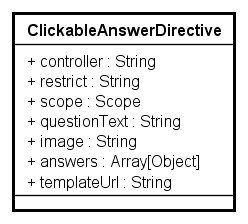
\includegraphics[scale=0.5,keepaspectratio]{UML/Classi/Front-End/QuizziPedia_Front-end_Templates_ClickableAnswerTemplate.png}
					\caption{QuizziPedia::Front-End::ModelViews::TopicKeywordsModelView}
				\end{figure} \FloatBarrier
				
				\begin{itemize}
					\item \textbf{Descrizione}: classe di tipo modelview la cui istanziazione è contenuta all'interno della variabile di ambiente \$scope di \textit{Angular.js\ped{G}}. All'interno di essa sono presenti le variabili e i metodi necessari per il \textit{Two-Way Data-Binding\ped{G}} tra la view \texttt{CreateQuestionnaireView} e il controller \texttt{KeywordsController};
					\item \textbf{Utilizzo}: viene utilizzata per effettuare il \textit{Two-Way Data-Binding\ped{G}} tra la view \texttt{CreateQuestionnaireView} e il controller \texttt{KeywordsController} rendendo disponibili variabili e metodi;
					\item \textbf{Relazioni con altre classi}: 
					\begin{itemize}
						\item \textit{IN} \texttt{CreateQuestionnaireView}: view per la creazione del questionario; 
						\item \textit{IN} \texttt{KeywordsController}: questa classe permette di gestire il recupero delle parole chiave di un questionario;
					\end{itemize}
					\item \textbf{Attributi}: 
					\begin{itemize}
						\item ;
					\end{itemize}
					\item \textbf{Metodi}: 
					\begin{itemize}
						\item ;
					\end{itemize}
				\end{itemize}
				
					
	\paragraph{QuizziPedia::Front-End::ModelViews::LoginModelView}
	
	\label{QuizziPedia::Front-End::ModelViews::LoginModelView}
	
	\begin{figure}[ht]
		\centering
		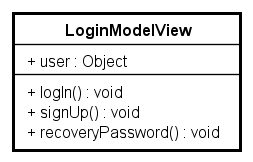
\includegraphics[scale=0.80,keepaspectratio]{UML/Classi/Front-End/QuizziPedia_Front-end_ModelView_LoginModelView.png}
		\caption{QuizziPedia::Front-End::ModelViews::LoginModelView}
	\end{figure} \FloatBarrier
	
	\begin{itemize}
		\item \textbf{Descrizione}: classe di tipo modelview la cui istanziazione è contenuta all'interno della variabile di ambiente \$scope di \textit{Angular.js\ped{G}}. All'interno di essa sono presenti le variabili e i metodi necessari per il \textit{Two-Way Data-Binding\ped{G}} tra la view \texttt{LoginView} e il controller \texttt{LoginController};
		\item \textbf{Utilizzo}: viene utilizzata per effettuare il \textit{Two-Way Data-Binding\ped{G}} tra la view \texttt{LoginView} e il controller \texttt{LoginController} rendendo disponibili variabili e metodi;
		\item \textbf{Relazioni con altre classi}: 
		\begin{itemize}
			\item \textit{OUT} \texttt{LoginView}: view contenente le form necessarie per effettuare il login. Contiene inoltre un link alla pagina di registrazione e uno alla pagina per il recupero della password; 
			\item \textit{OUT} \texttt{LoginController}: questa classe permette di gestire l'autenticazione dell'utente al sistema;
		\end{itemize}
		\item \textbf{Attributi}: 
		\begin{itemize}
				\item \texttt{+ user: Object} \\ Campo dati contenente due attributi: \texttt{username: String} e \texttt{password: String}.
		\end{itemize}
		\item \textbf{Metodi}: 
		\begin{itemize}
			\item \texttt{+} \texttt{logIn(): void} \\
			Metodo che richiama il metodo \texttt{Login} del service \texttt{AuthService} passandogli \texttt{username} e \texttt{password}. Nel caso di buona riuscita dell'operazione viene effettuato il redirect alla homepage dell'applicazione. Nel caso in cui invece avvenga un errore, viene mostrato a video il messaggio di errore;
			\item \texttt{+} \texttt{signUp(): void} \\
			Metodo che gestisce l’evento click sul pulsante di registrazione. Effettua il redirect alla pagina di registrazione;
			\item \texttt{+} \texttt{recoveryPassword(): void} \\
			Metodo che gestisce l’evento click sul pulsante di recupero password. Effettua il redirect alla pagina per il recupero della password; 
		\end{itemize}
	\end{itemize}
	
	
	\paragraph{QuizziPedia::Front-End::ModelViews::MenuBarModelView}

\label{QuizziPedia::Front-End::ModelViews::MenuBarModelView}

\begin{figure}[ht]
	\centering
	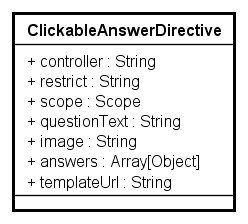
\includegraphics[scale=0.5,keepaspectratio]{UML/Classi/Front-End/QuizziPedia_Front-end_Templates_ClickableAnswerTemplate.png}
	\caption{QuizziPedia::Front-End::ModelViews::MenuBarModelView}
\end{figure} \FloatBarrier

\begin{itemize}
	\item \textbf{Descrizione}: classe di tipo modelview la cui istanziazione è contenuta all'interno della variabile di ambiente \$scope di \textit{Angular.js\ped{G}}. All'interno di essa sono presenti le variabili e i metodi necessari per il \textit{Two-Way Data-Binding\ped{G}} tra la view \texttt{Index} e il controller \texttt{MenuBarController};
	\item \textbf{Utilizzo}: viene utilizzata per effettuare il \textit{Two-Way Data-Binding\ped{G}} tra la view \texttt{Index} e il controller \texttt{MenuBarController} rendendo disponibili variabili e metodi;
	\item \textbf{Relazioni con altre classi}: 
	\begin{itemize}
		\item \textit{OUT} \texttt{LoginBarDirective}: directive contenente il componente che permette di effettuare il redirect alla pagina di login;
		\item \textit{OUT} \texttt{SignUpBarDirective}: directive contenente il componente che permette di effettuare il redirect alla pagina di registrazione;
		\item \textit{OUT} \texttt{UserBarDirective}: directive contenente il componente che permette di effettuare il redirect alla pagina di visualizzazione del profilo utente personale;
		\item \textit{OUT} \texttt{ProfileManagementBarDirective}: directive contenente il componente che permette di effettuare il redirect alla pagina di gestione del profilo;
		\item \textit{OUT} \texttt{QuestionsManagementBarDirective}: directive contenente il componente che permette di effettuare il redirect alla pagina di gestione delle domande;
		\item \textit{OUT} \texttt{LogoutBarDirective}: directive contenente il componente che permette di effettuare il logout;
		\item \textit{OUT} \texttt{QuestionnaireManagementBarDirective}: directive contenente il componente che permette di effettuare il redirect alla pagina di gestione dei questionari;
		\item \textit{OUT} \texttt{MenuBarController}: questa classe permette di gestire il menù fisso per ogni pagina.
	\end{itemize}
	\item \textbf{Attributi}: 
	\begin{itemize}
		\item \texttt{+ username: String} \\ Attributo che conterrà l'username dell'utente.
	\end{itemize}
	\item \textbf{Metodi}: 
	\begin{itemize}
		\item \texttt{+} \texttt{logOut(): void} \\
		Metodo che richiama il metodo \texttt{logOut} del service \texttt{AuthService} passandogli lo \texttt{username}. Prima di effettuare questa operazione viene mostrato a video un messaggio di conferma per il proseguo dell'operazione; 
		\item \texttt{+} \texttt{logIn(): void} \\
		Metodo che gestisce l’evento click sul pulsante per effettuare il login. Effettua il redirect alla pagina per effettuare il login; 
		\item \texttt{+} \texttt{signUp(): void} \\
		Metodo che gestisce l’evento click sul pulsante per effettuare la registrazione. Effettua il redirect alla pagina per effettuare la registrazione; 
		\item \texttt{+} \texttt{goToUserPage(): void} \\
		Metodo che gestisce l’evento click sul pulsante di visualizzazione della pagina utente. Effettua il redirect alla pagina di visualizzazione della pagina utente; 
		\item \texttt{+} \texttt{goToUserManagemetPage(): void} \\
		Metodo che gestisce l’evento click sul pulsante di gestione del profilo utente. Effettua il redirect alla pagina di gestione del profilo utente; 
		\item \texttt{+} \texttt{goToQuestionsManagementPage(): void} \\
		Metodo che gestisce l’evento click sul pulsante di gestione delle domande. Effettua il redirect alla pagina di gestione delle domande; 
		\item \texttt{+} \texttt{goToQuizManagementPage(): void} \\
		Metodo che gestisce l’evento click sul pulsante di gestione dei questionari. Effettua il redirect alla pagina di gestione dei questionari;
		\item \texttt{+ \$on('\$routeChangeStart': String, callback: function): void} \\
		Metodo che cattura i cambiamenti dell'url e che richiede al \texttt{MenuBarModel} le giuste direttive da inserire in \texttt{MenuBarDirective}. \\
		\textbf{Parametri};
		\begin{itemize}
			\item \texttt{'\$routeChangeStart': String}	\\ Servizio offerto da \textit{Angular.js\ped{G}} per catturare gli eventi sulla barra degli URL;
			\item \texttt{callback: function}	\\ Funzione di callback per gestire i cambiamenti della barra degli indirizzi.
		\end{itemize}
	\end{itemize}
\end{itemize}


	\paragraph[QuizziPedia::Front-End::ModelViews\\::MultipleQuestionsModelView]{QuizziPedia::Front-End::ModelViews::MultipleQuestionsModelView}
\begin{figure} [ht]
	\centering
	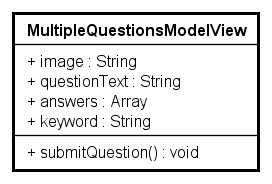
\includegraphics[scale=0.80]{UML/Classi/Front-End/QuizziPedia_Front-end_ModelView_MultipleQuestionsModelView.png}
	\caption{QuizziPedia::Front-End::ModelViews::MultipleQuestionsModelView}
\end{figure} \FloatBarrier
\begin{itemize}
	\item \textbf{Descrizione}: classe di tipo modelview la cui istanziazione è contenuta all'interno della variabile di ambiente \texttt{\$scope} di \textit{Angular\ped{G}}. All'interno di essa sono presenti le variabili e i metodi necessari per il \textit{Two-Way Data-Binding\ped{G}} tra la \textit{view\ped{G}} \texttt{MultipleQuestionsView} e il \textit{controller\ped{G}} \texttt{MultipleQuestionsController}; 
	\item \textbf{Utilizzo}: viene utilizzata per effettuare il \textit{Two-Way Data-Binding\ped{G}} tra la \textit{view\ped{G}} \\\texttt{MultipleQuestionsView} e il \textit{controller\ped{G}} \texttt{MultipleQuestionsController} rendendo disponibili variabili e metodi;
	\item \textbf{Relazioni con altre classi}:
	\begin{itemize}
		\item \textbf{IN \texttt{MultipleQuestionsView}}: \textit{view\ped{G}} contenente le direttive per creare una domanda a risposta multipla; 
		\item \textbf{IN \texttt{MultipleQuestionsController}}: questa classe permette di gestire la creazione e la modifica di una domanda a risposta multipla.
	\end{itemize}
	\item \textbf{Attributi}:
	\begin{itemize}
		\item \texttt{+ image: String} \\ Attributo contenete l'URL dell'immagine caricata dall'utente;
		\item \texttt{+ questionText: String} \\ Attributo contenente il testo della domanda;
		\item \texttt{+ answers: Array}\\ \texttt{array} che contiene coppie di valori. Queste coppie sono formate da:
		\begin{itemize}
			\item \texttt{type: String} \\ Indica la tipologia della risposta;
			\item \texttt{text: String} \\ Contiene il testo dell'affermazione;
			\item \texttt{url: String} \\ Rappresenta l'immagine della risposta;
			\item \texttt{attributesForTForMultiple: Mixed} \\ Contiene i seguenti attributi:
			\begin{enumerate}
				\item \texttt{isItRight: Boolean} \\ Contiene se la risposta è vera o falsa.
			\end{enumerate}
		\end{itemize}
		\item \texttt{+ keyword: String} \\ Attributo contenente la keyword associata alla domanda/questionario.
	\end{itemize}
	\item \textbf{Metodi}:
	\begin{itemize}
		\item \texttt{+ submitQuestion(): void}\\ 
		Metodo che gestisce l’evento click sul pulsante di conferma sulla domanda. Raccoglie i dati dal modelview e li manda al server attraverso \texttt{QuestionService}. Poi verrà effettuato il redirect alla pagina di gestione delle domande oppure al questionario che si stava creando.
	\end{itemize}
\end{itemize}


	\paragraph{QuizziPedia::Front-End::ModelViews::PasswordForgotModelView}
	
	\label{QuizziPedia::Front-End::ModelViews::PasswordForgotModelView}
	
	\begin{figure}[ht]
		\centering
		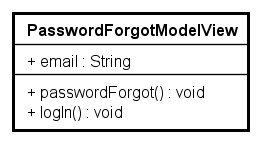
\includegraphics[scale=0.8,keepaspectratio]{UML/Classi/Front-End/QuizziPedia_Front-end_ModelView_PasswordForgotModelView.png}
		\caption{QuizziPedia::Front-End::ModelViews::PasswordForgotModelView}
	\end{figure} \FloatBarrier
	
	\begin{itemize}
		\item \textbf{Descrizione}: classe di tipo modelview la cui istanziazione è contenuta all'interno della variabile di ambiente \texttt{\$scope} di \textit{Angular\ped{G}}. All'interno di essa sono presenti le variabili e i metodi necessari per il \textit{Two-Way Data-Binding\ped{G}} tra la \textit{view\ped{G}} \texttt{PasswordForgotView} e il \textit{controller\ped{G}} \texttt{PasswordForgotController};
		\item \textbf{Utilizzo}: viene utilizzata per effettuare il \textit{Two-Way Data-Binding\ped{G}} tra la \textit{view\ped{G}} \texttt{PasswordForgotView} e il \textit{controller\ped{G}} \texttt{PasswordForgotController} rendendo disponibili variabili e metodi;
		\item \textbf{Relazioni con altre classi}: 
		\begin{itemize}
			\item \textbf{OUT \texttt{PasswordForgotView}}: \textit{view\ped{G}} contenente le form necessarie per il recupero della password dimenticata; 
			\item \textbf{OUT \texttt{PasswordForgotController}}: questa classe permette di gestire il ripristino della password dimenticata.
		\end{itemize}
		\item \textbf{Attributi}: 
		\begin{itemize}
			\item \texttt{+ email: String} \\ Campo dati contenente l'email per il recupero password.
		\end{itemize}
		\item \textbf{Metodi}: 
		\begin{itemize}
			\item \texttt{+ passwordForgot(email: String): void} \\
			Metodo che richiama il metodo \texttt{passwordForgot} del service \texttt{AuthService} passandogli il parametro \texttt{email}. Nel caso di buona riuscita dell'operazione, viene mostrato un messaggio di successo il cui corpo contiene anche un bottone per effettuare il redirect alla pagina di login. Nel caso in cui invece avvenga un errore, viene mostrato a video il messaggio di errore;
			\item \texttt{+ logIn(): void} \\
			Metodo che gestisce l’evento click sul pulsante di login. Effettua il redirect alla pagina di login.
		\end{itemize}
	\end{itemize}
	
	
		\paragraph{QuizziPedia::Front-End::ModelViews::ProfileManagementModelView}
	
	\label{QuizziPedia::Front-End::ModelViews::ProfileManagementModelView}
	
	\begin{figure}[ht]
		\centering
		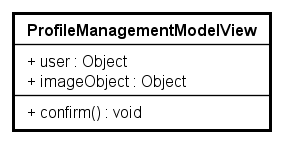
\includegraphics[scale=0.80,keepaspectratio]{UML/Classi/Front-End/QuizziPedia_Front-end_ModelView_ProfileManagementModelView.png}
		\caption{QuizziPedia::Front-End::ModelViews::ProfileManagementModelView}
	\end{figure} \FloatBarrier
	
	\begin{itemize}
		\item \textbf{Descrizione}: classe di tipo modelview la cui istanziazione è contenuta all'interno della variabile di ambiente \$scope di \textit{Angular.js\ped{G}}. All'interno di essa sono presenti le variabili e i metodi necessari per il \textit{Two-Way Data-Binding\ped{G}} tra la view \texttt{ProfileManagementView} e il controller \texttt{ProfileManagementController};
		\item \textbf{Utilizzo}: viene utilizzata per effettuare il \textit{Two-Way Data-Binding\ped{G}} tra la view \texttt{ProfileManagementView} e il controller \texttt{ProfileManagementController} rendendo disponibili variabili e metodi;
		\item \textbf{Relazioni con altre classi}: 
		\begin{itemize}
			\item \textit{OUT} \texttt{ProfileManagementView}: view contenente i dati personali che un utente può modificare dopo essersi registrato al sistema; 
			\item \textit{OUT} \texttt{ProfileManagementController}: questa classe permette di gestire il profilo personale di un utente;
		\end{itemize}
		\item \textbf{Attributi}: 
		\begin{itemize}
			\item \texttt{+ user: Object} \\ Campo dati contenente i seguenti attributi: \texttt{name: String}, \texttt{surname: String}, \texttt{email: String}, \texttt{image: String}, \texttt{password: String} e \texttt{passwordCheck: String};
			\item \texttt{+ imageObject: Object} \\ Oggetto contenente i seguenti attributi: \texttt{+ imageUrl: String}, \texttt{+ image: Object};
		\end{itemize}
		\item \textbf{Metodi}: 
		\begin{itemize}
			\item \texttt{+} \texttt{confirm(user: Object, imageObject: Object): void} \\
			Metodo che gestisce l’evento click sul pulsante di conferma modifica. Aggiorna, in caso di modifiche accettate da sistema, l'oggetto locale \texttt{UserDetailsModel}. Inoltre, utilizzando il metodo dell'\texttt{UserDetailsService}, aggiorna anche nel server i dati dell'utente.
		\end{itemize}
	\end{itemize}	


	\paragraph[QuizziPedia::Front-End::ModelViews\\::QuestionnaireDetailsModelView]{QuizziPedia::Front-End::ModelViews::QuestionnaireDetailsModelView}
	
	\label{QuizziPedia::Front-End::ModelViews::QuestionnaireDetailsModelView}
	
	\begin{figure}[ht]
		\centering
		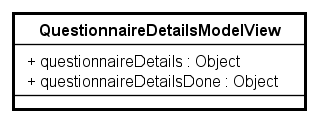
\includegraphics[scale=0.5,keepaspectratio]{UML/Classi/Front-End/QuizziPedia_Front-end_ModelView_QuestionnaireDetailsModelView.png}
		\caption{QuizziPedia::Front-End::ModelViews::QuestionnaireDetailsModelView}
	\end{figure} \FloatBarrier
	
	\begin{itemize}
		\item \textbf{Descrizione}: classe di tipo modelview la cui istanziazione è contenuta all'interno della variabile di ambiente \texttt{\$scope} di \textit{Angular\ped{G}}. All'interno di essa sono presenti le variabili e i metodi necessari per il \textit{Two-Way Data-Binding\ped{G}} tra la \textit{view\ped{G}} \texttt{UserView} e il \textit{controller\ped{G}} \texttt{QuestionnaireDetailsController};
		\item \textbf{Utilizzo}: viene utilizzata per effettuare il \textit{Two-Way Data-Binding\ped{G}} tra la \textit{view\ped{G}} \texttt{UserView} e il \textit{controller\ped{G}} \texttt{QuestionnaireDetailsController} rendendo disponibili variabili e metodi;
		\item \textbf{Relazioni con altre classi}: 
		\begin{itemize}
			\item \textbf{OUT \texttt{QuestionnaireDetailsDirective}}: rappresenta il componente grafico che permette all'utente di visualizzare la lista di questionari che può compilare;
			\item \textbf{OUT \texttt{QuestionnaireDetailsDoneDirective}}: rappresenta il componente grafico che permette all'utente di visualizzare la lista di questionari che ha già compilato e di conseguenza vederne le valutazioni;
			\item \textbf{OUT \texttt{QuestionnaireDetailsController}}: questa classe permette di gestire i dettagli di un questionario.
		\end{itemize}
		\item \textbf{Attributi}: 
		\begin{itemize}
			\item \texttt{+ questionnaireDetails: Object} \\ Oggetto contenente i seguenti campi dati:
			\begin{itemize}
				\item \texttt{name: String}\\ Nome del questionario;
				\item \texttt{author: String}\\ Autore del questionario;
				\item \texttt{topic: String}\\ Argomento del questionario;
				\item \texttt{keywords: Array[String]}\\ Parole chiave del questionario.
			\end{itemize}
			\item \texttt{+ questionnaireDetailsDone: Object} \\ Oggetto contenente i seguenti campi dati:
			\begin{itemize}
				\item \texttt{name: String}\\ Nome del questionario;
				\item \texttt{author: String}\\ Autore del questionario;
				\item \texttt{topic: String}\\ Argomento del questionario;
				\item \texttt{keywords: Array[String]}\\ Parole chiave del questionario;
				\item \texttt{judgement: Number} \\ Campo che indica il risultato del questionario.
			\end{itemize}
		\end{itemize}
	\end{itemize}
	
		
	\paragraph[QuizziPedia::Front-End::ModelViews\\::QuestionnaireManagementModelView]{QuizziPedia::Front-End::ModelViews::QuestionnaireManagementModelView}
	
	\label{QuizziPedia::Front-End::ModelViews::QuestionnaireManagementModelView}
	
	\begin{figure}[ht]
		\centering
		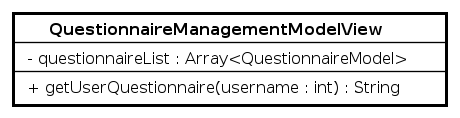
\includegraphics[scale=0.8,keepaspectratio]{UML/Classi/Front-End/QuizziPedia_Front-end_ModelView_QuestionnaireManagementModelView.png}
		\caption{QuizziPedia::Front-End::ModelViews::QuestionnaireManagementModelView}
	\end{figure} \FloatBarrier
	
	\begin{itemize}
		\item \textbf{Descrizione}: classe di tipo modelview la cui istanziazione è contenuta all'interno della variabile di ambiente \texttt{\$scope} di \textit{Angular\ped{G}}. All'interno di essa sono presenti le variabili e i metodi necessari per il \textit{Two-Way Data-Binding\ped{G}} tra la \textit{view\ped{G}} \texttt{QuestionnaireManagementView} e il \textit{controller\ped{G}} \texttt{QuestionnaireManagementController};
		\item \textbf{Utilizzo}: viene utilizzata per effettuare il \textit{Two-Way Data-Binding\ped{G}} tra la \textit{view\ped{G}} \texttt{QuestionnaireManagementView} e il \textit{controller\ped{G}} \texttt{QuestionnaireManagementController} rendendo disponibili variabili e metodi;
		\item \textbf{Relazioni con altre classi}: 
		\begin{itemize}
			\item \textbf{IN \texttt{QuestionnaireManagementView}}: \textit{view\ped{G}} principale per la gestione dei questionari; 
			\item \textbf{IN \texttt{QuestionnaireManagementController}}: questa classe permette di gestire tutti i questionari creati da un utente;
		\end{itemize}
		\item \textbf{Attributi}: 
		\begin{itemize}
			\item \texttt{- questionnaireList: Array} \\ \texttt{array} contenente la lista dei questionari creati; ogni questionario sarà rappresentato come un oggetto.
		\end{itemize}
		\item \textbf{Metodi}:
		\begin{itemize}
				\item \texttt{+ getUserQuestionnaire(username: String) QuestionnaireModel[]}: \\Metodo che ritorna tutti i questionari creati da un utente in un array di QuestionnaireModel.
				\textbf{Parametri}:
				\begin{itemize}
					\item \texttt{username: String}\\ 
					Parametro che indica l'identificativo dell'utente del quale vogliamo scaricare tutti i questionari.
				\end{itemize}
		\end{itemize} 
	\end{itemize}
	
	
	\paragraph{QuizziPedia::Front-End::ModelViews::QuestionnaireQuestionsManagementModelView}
					
					\label{QuizziPedia::Front-End::ModelViews::QuestionnaireQuestionsManagementModelView}
					
					\begin{figure}[ht]
						\centering
						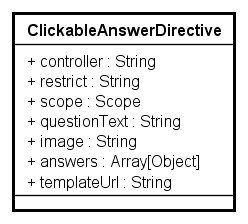
\includegraphics[scale=0.5,keepaspectratio]{UML/Classi/Front-End/QuizziPedia_Front-end_Templates_ClickableAnswerTemplate.png}
						\caption{QuizziPedia::Front-End::ModelViews::QuestionnaireQuestionsManagementModelView}
					\end{figure} \FloatBarrier
					
					\begin{itemize}
						\item \textbf{Descrizione}: classe di tipo modelview la cui istanziazione è contenuta all'interno della variabile di ambiente \$scope di \textit{Angular.js\ped{G}}. All'interno di essa sono presenti le variabili e i metodi necessari per il \textit{Two-Way Data-Binding\ped{G}} tra la view \texttt{QuestionnaireQuestionsManagementView} e il controller \texttt{QuestionnaireQuestionsManagementController};
						\item \textbf{Utilizzo}: viene utilizzata per effettuare il \textit{Two-Way Data-Binding\ped{G}} tra la view \texttt{QuestionnaireQuestionsManagementView} e il controller \texttt{QuestionnaireQuestionsManagementController} rendendo disponibili variabili e metodi;
						\item \textbf{Relazioni con altre classi}: 
						\begin{itemize}
							\item \textit{IN} \texttt{CreateQuestionnaireView}: view per la creazione del questionario; 
							\item \textit{IN} \texttt{QuestionnaireQuestionsManagementController}: questa classe permette di gestire il recupero delle parole chiave di un questionario;
						\end{itemize}
						\item \textbf{Attributi}: 
						\begin{itemize}
							\item ;
						\end{itemize}
						\item \textbf{Metodi}: 
						\begin{itemize}
							\item ;
						\end{itemize}
					\end{itemize}
					
						
							
	\paragraph[QuizziPedia::Front-End::ModelViews\\::QuestionsManagementModelView]{QuizziPedia::Front-End::ModelViews::QuestionsManagementModelView}

\label{QuizziPedia::Front-End::ModelViews::QuestionsManagementModelView}

\begin{figure}[ht]
	\centering
	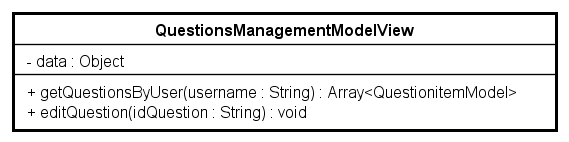
\includegraphics[scale=0.8,keepaspectratio]{UML/Classi/Front-End/QuizziPedia_Front-end_ModelView_QuestionsManagementModelView.png}
	\caption{QuizziPedia::Front-End::ModelViews::QuestionsManagementModelView}
\end{figure} \FloatBarrier

\begin{itemize}
	\item \textbf{Descrizione}: classe di tipo modelview la cui istanziazione è contenuta all'interno della variabile di ambiente \texttt{\$scope} di \textit{Angular\ped{G}}. All'interno di essa sono presenti le variabili e i metodi necessari per il \textit{Two-Way Data-Binding\ped{G}} tra la \textit{view\ped{G}} \texttt{QuestionsManagementView} e il \textit{controller\ped{G}} \texttt{QuestionsManagementController};
	\item \textbf{Utilizzo}: viene utilizzata per effettuare il \textit{Two-Way Data-Binding\ped{G}} tra la \textit{view\ped{G}} \\\texttt{QuestionsManagementView} e il \textit{controller\ped{G}} \texttt{QuestionsManagementController} rendendo disponibili variabili e metodi;
	\item \textbf{Relazioni con altre classi}: 
	\begin{itemize}
		\item \textbf{IN \texttt{QuestionsManagementView}}: \textit{view\ped{G}} contenente l’elenco delle domande create; 
		\item \textbf{IN \texttt{QuestionsManagementController}}: questa classe permette di gestire le domande create dall’utente e di crearne di nuove.
	\end{itemize}
	\item \textbf{Attributi}: 
	\begin{itemize}
		\item \texttt{- data: Object} \\ Oggetto contenete le informazioni da mostrare nell'anteprima della domanda.
	\end{itemize}
	\item \textbf{Metodi}: 
	\begin{itemize}
			\item \texttt{+ getQuestionsByUser(username: String) : Array<QuestionItemModel>} \\ 
			Metodo che acquisisce le domande create dall'utente attraverso il \texttt{QuestionService}.\\
			\textbf{Parametri}:
			\begin{itemize}
				\item \texttt{username: String} \\
				Parametro di tipo \texttt{String} contenente l'username dell'utente.
			\end{itemize}
			\item \texttt{+ editQuestion(idQuestion: String) : Void} \\ 
			Metodo che gestisce l’evento click sul pulsante per modificare la domanda. Effettua il redirect alla pagina di modifica della domanda. \\
			\textbf{Parametri}:
			\begin{itemize}
				\item \texttt{idQuestion: username} \\
				Parametro di tipo \texttt{String} contenente l'id della domanda da modificare.
			\end{itemize}
	\end{itemize}
\end{itemize}	


	\paragraph{QuizziPedia::Front-End::ModelViews::QuestionsModelView}

\label{QuizziPedia::Front-End::ModelViews::QuestionsModelView}

\begin{figure}[ht]
	\centering
	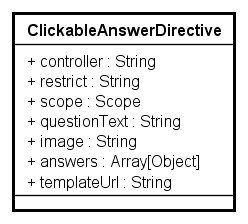
\includegraphics[scale=0.5,keepaspectratio]{UML/Classi/Front-End/QuizziPedia_Front-end_Templates_ClickableAnswerTemplate.png}
	\caption{QuizziPedia::Front-End::ModelViews::QuestionsModelView}
\end{figure} \FloatBarrier

\begin{itemize}
	\item \textbf{Descrizione}: classe di tipo modelview la cui istanziazione è contenuta all'interno della variabile di ambiente \$scope di \textit{Angular.js\ped{G}}. All'interno di essa sono presenti le variabili e i metodi necessari per il \textit{Two-Way Data-Binding\ped{G}} tra le directive che compongono dinamicamente la vista della domanda e il controller \texttt{QuestionsController};
	\item \textbf{Utilizzo}: viene utilizzata per effettuare il \textit{Two-Way Data-Binding\ped{G}} tra le directive che compongono dinamicamente la vista della domanda e il controller \texttt{QuestionsController} rendendo disponibili variabili e metodi;
	\item \textbf{Relazioni con altre classi}: 
	\begin{itemize} 
		\item \textit{OUT} \texttt{QuestionsController}: questa classe permette di gestire il recupero delle domande per poterle stampare nella modalità allenamento;
		\item \textit{OUT} \texttt{ClickableAnswerDirective}: rappresenta il componente grafico che permette all'utente di visualizzare la domanda ad area cliccabile nell'immagine. Viene visualizzato dinamicamente all'interno delle views TrainingView e FillingQuestionnaireView mediante il controller QuestionsController;
		\item \textit{OUT} \texttt{EmptySpaceAnswerDirective}: rappresenta il componente grafico che permette all'utente di visualizzare l'esercizio a riempimento di spazi vuoti. Viene visualizzato dinamicamente all'interno delle views TrainingView e FillingQuestionnaireView mediante il controller QuestionsController;
		\item \textit{OUT} \texttt{HeaderTextQuestionDirective}: rappresenta il componente grafico che presenta all'utente l'argomento, le parole chiave e il numero di domande complessive. Viene visualizzato dinamicamente all'interno delle views TrainingView e FillingQuestionnaireView mediante il controller QuestionsController;
		\item \textit{OUT} \texttt{LinkingAnswerDirective}: rappresenta il componente grafico che permette all'utente di visualizzare la domanda di collegamento. Viene visualizzato dinamicamente all'interno delle views TrainingView e FillingQuestionnaireView mediante il controller QuestionsController;
		\item \textit{OUT} \texttt{MultipleChoiceAnswerDirective}: rappresenta il componente grafico che permette all'utente di visualizzare la domanda a risposta multipla. Viene visualizzato dinamicamente all'interno delle views TrainingView e FillingQuestionnaireView mediante il controller QuestionsController;
		\item \textit{OUT} \texttt{SortImagesAnswerDirective}: rappresenta il componente grafico che permette all'utente di visualizzare la domanda ad ordinamento di immagini. Viene visualizzato dinamicamente all'interno delle views TrainingView e FillingQuestionnaireView mediante il controller QuestionsController;
		\item \textit{OUT} \texttt{SortTextAnswerDirective}: rappresenta il componente grafico che permette all'utente di visualizzare la domanda ad ordinamento di stringhe. Viene visualizzato dinamicamente all'interno delle views TrainingView e FillingQuestionnaireView mediante il controller QuestionsController;
		\item \textit{OUT} \texttt{TrueFalseAnswareDirective}: rappresenta il componente grafico che permette all'utente di visualizzare la domanda vero e falso. Viene visualizzato dinamicamente all'interno delle views TrainingView e FillingQuestionnaireView mediante il controller QuestionsController;	
		\item \textit{OUT} \texttt{TrainingView}: view principale della modalità allenamento, conterrà i vari templates di ogni domanda dell'allenamento.				
	\end{itemize}
	\item \textbf{Attributi}: 
	\begin{itemize}
		\item \texttt{+ piecesOfQuestion: Array[Object]} \\
		Questo attributo è un \texttt{array} di \texttt{Object} contenente la domanda da visualizzare dinamicamente attraverso le direttive all'interno le direttive di allenamento e di compilazione dei questionari;
		\item \texttt{+ objAnswer: Array[Object]} \\
		Questo attributo è un \texttt{array} di \texttt{Object} contenente le risposte date fino a quel momento dall'utente in una domanda. L'\texttt{Object} è così formato: \\
		\begin{itemize}
			\item \texttt{+ typeQuestion: String} \\
			Questo attributo rappresenta il tipo della domanda;
			\item \texttt{+ answerGiven: Array[String]} \\
			Questo attributo rappresenta le riposte scelte dall'utente fino a quel momento. Può essere creato con una funzione di \texttt{callback}.
		\end{itemize}
	\end{itemize}
	\item \textbf{Metodi}: 
	\begin{itemize}
		\item \texttt{+} \texttt{addAnswer(index: Number, typeQuestion: String, answerGiven: Array[String]): void} \\
		Metodo che gestisce l'evento di selezione delle risposte. \\
		\textbf{Parametri}:
		\begin{itemize}
			\item \texttt{index: Number} \\
			Parametro contenente l'indice della risposta di cui si vuole tenere traccia. Rappresenta anche l'indice dell'\texttt{array objAswer} in cui verrà inserito l'oggetto delle risposte date;
			\item \texttt{typeQuestion: String} \\
			Parametro contenente una stringa la quale indica la tipologia della domanda;
			\item \texttt{answerGiven: Array[String]} \\
			Parametro contenente l'array di risposte date dall'utente aggiornato all'ultima iterazione.
		\end{itemize};
		\item \texttt{+} \texttt{answerGiven(index: Number): Array[String]} \\
		Metodo di supporto che ritorna un \texttt{array} di stringhe contenente le risposte date. Si occupa di recuperare le risposte date nelle domande vero/falso, risposta multipla e ad area cliccabile.\\
		\textbf{Parametri}:
		\begin{itemize}
			\item \texttt{index: Number} \\
			Parametro contenente l'indice della risposta di cui si vuole raccogliere le risposte date. 
		\end{itemize}
		\item \texttt{+} \texttt{orderChosen(index: Number): Array[String]} \\
		Metodo di supporto che ritorna un \texttt{array} di stringhe contenente le risposte date. Si occupa di recuperare le risposte date nelle domande ad ordinamento e di riempimento di spazi.\\
		\textbf{Parametri}:
		\begin{itemize}
			\item \texttt{index: Number} \\
			Parametro contenente l'indice della risposta di cui si vuole raccogliere le risposte date. 
		\end{itemize}
		\item \texttt{+} \texttt{linkingMade(index: Number): Array[String]} \\
		Metodo di supporto che ritorna un \texttt{array} di stringhe contenente le risposte date. Si occupa di recuperare le risposte date nelle domande a collegamento.\\
		\textbf{Parametri}:
		\begin{itemize}
			\item \texttt{index: Number} \\
			Parametro contenente l'indice della risposta di cui si vuole raccogliere le risposte date. 
		\end{itemize}
		\item \texttt{+} \texttt{loadNewQuestionBy(topic: String, keywords: Array[String], level: Number): void} \\
		Metodo che gestisce l'evento per scaricare una nuova domanda in base ai parametri passati. Evoca l'evento per inserire la domanda in \texttt{TrainingModelView}. \\
		\textbf{Parametri}:
		\begin{itemize}
			\item \texttt{topic: String} \\
			Parametro contenente l'argomento della domanda;
			\item \texttt{keywords: Array[String]} \\
			Parametro contenente un\texttt{array} di stringhe che rappresenta le keywords scelte per l'allenamento;
			\item \texttt{level: Number} \\
			Parametro contenente il livello dell'utente.
		\end{itemize}
		\item \texttt{+} \texttt{loadNewQuestion(question: QuestionItemModel): void} \\
		Metodo che gestisce l'evento per visualizzare una nuova domanda. \\
		\textbf{Parametri}:
		\begin{itemize}
			\item \texttt{question: QuestionItemModel} \\
			Parametro contenente un riferimento all'oggetto di tipo \texttt{QuestionItemModel}.
		\end{itemize}
		\item \texttt{+} \texttt{checkAnswer(): boolean} \\ 
		Metodo che controlla che le risposte date siano corrette.
	\end{itemize}
\end{itemize}

	
	\paragraph{QuizziPedia::Front-End::ModelViews::QuizEventModelView}
							
\label{QuizziPedia::Front-End::ModelViews::QuizEventModelView}

\begin{figure}[ht]
	\centering
	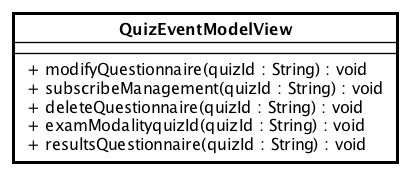
\includegraphics[scale=0.5,keepaspectratio]{UML/Classi/Front-End/QuizziPedia_Front-end_ModelView_QuizEventModelView.png}
	\caption{QuizziPedia::Front-End::ModelViews::QuizEventModelView}
\end{figure} \FloatBarrier

\begin{itemize}
	\item \textbf{Descrizione}: classe di tipo modelview la cui istanziazione è contenuta all'interno della variabile di ambiente \texttt{\$scope} di \textit{Angular\ped{G}}. All'interno di essa sono presenti le variabili e i metodi necessari per il \textit{Two-Way Data-Binding\ped{G}} tra le \textit{directives\ped{G}}\\ \texttt{EliminationAndModifyDirective}, \texttt{ExamModalityDirective} e \texttt{QuestionnaireResultsDirective} e il \textit{controller\ped{G}} \texttt{QuizEventController};
	\item \textbf{Utilizzo}: viene utilizzata per effettuare il \textit{Two-Way Data-Binding\ped{G}} tra le \textit{directives\ped{G}}\\ \texttt{EliminationAndModifyDirective}, \texttt{ExamModalityDirective} e \texttt{QuestionnaireResultsDirective} e il \textit{controller\ped{G}} \texttt{QuizEventController} rendendo disponibili variabili e metodi;
	\item \textbf{Relazioni con altre classi}: 
	\begin{itemize}
		\item \textbf{OUT \texttt{EliminationAndModifyDirective}}: componente grafico contenente i bottoni per eliminare o modificare un questionario;
		\item \textbf{OUT \texttt{ExamModalityDirective}}: \textit{directive\ped{G}} contenente i componenti grafici per attivare la modalità esame su un questionario e gestire le iscrizioni; 
		\item \textbf{OUT \texttt{QuestionnaireResultsDirective}}: rappresenta il componente grafico che permette all'utente autenticato pro di vedere i risultati di chi ha compilato il questionario. Tale componente è contenuto nella lista dei questionari abilitati alla compilazione. \'E possibile accedere alla lista dei risultati azionando l'evento ad esso collegato; 
		\item \textbf{OUT \texttt{QuizEventController}}: questa classe permette di reagire ai comandi dell'utente durante la gestione dei suoi questionari.
	\end{itemize}
	\item \textbf{Metodi}: 
	\begin{itemize}
		\item \texttt{+ modifyQuestionnaire(quizId: String): void} \\
		Metodo che gestisce l'evento click sul pulsante di modifica questionario. Effettua il redirect alla pagina di gestione questionari.\\
		\textbf{Parametri}:
		\begin{itemize}
			\item \texttt{quizId: String}\\ 
			Parametro che indica l'identificativo univoco di un questionario.
		\end{itemize}
		\item \texttt{+ deleteQuestionnaire(quizId: String): void} \\
		Metodo che gestisce l'evento click sul pulsante di eliminazione questionario. Effettua il redirect alla pagina di gestione questionari.\\
		\textbf{Parametri}:  
		\begin{itemize}
			\item \texttt{quizId: String}\\
			Parametro che indica l'identificativo univoco di un questionario.
		\end{itemize}
		
		\item \texttt{+ subscribeManagement(quizId: String): void} \\
		Metodo che gestisce l'evento click sul pulsante di gestione iscrizioni. Effettua il redirect alla pagina di gestione iscrizioni.\\
		\textbf{Parametri}:
		\begin{itemize}
			\item \texttt{quizId: String}\\
			Parametro che indica l'identificativo univoco di un questionario.
		\end{itemize}
		
		\item \texttt{+ examModalityquizId: String(): void} \\
		Metodo che gestisce l'evento click sul pulsante di attivazione modalità esame. Effettua il redirect alla pagina di gestione questionari.
		\textbf{Parametri}:
		\begin{itemize}
			\item \texttt{quizId: String}\\ 
			Parametro che indica l'identificativo univoco di un questionario.
		\end{itemize}
		\item \texttt{+ resultsQuestionnaire(quizId: String): void} \\
		Metodo che gestisce l'evento click sul pulsante di allenamento. Effettua il redirect alla pagina di gestione questionari.
		\begin{itemize}
			\item \texttt{quizId: String}\\
			Parametro che indica l'identificativo univoco di un questionario.
		\end{itemize}   
	\end{itemize}
\end{itemize}
	\paragraph[QuizziPedia::Front-End::ModelViews\\::RegistrationManagementModelView]{QuizziPedia::Front-End::ModelViews::RegistrationManagementModelView}
	
	\label{QuizziPedia::Front-End::ModelViews::RegistrationManagementModelView}
	
	\begin{figure}[ht]
		\centering
		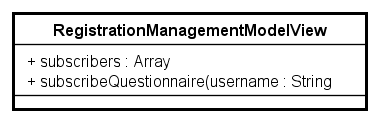
\includegraphics[scale=0.5,keepaspectratio]{UML/Classi/Front-End/QuizziPedia_Front-end_ModelView_RegistrationManagementModelView.png}
		\caption{QuizziPedia::Front-End::ModelViews::RegistrationManagementModelView}
	\end{figure} \FloatBarrier
	
	\begin{itemize}
		\item \textbf{Descrizione}: classe di tipo modelview la cui istanziazione è contenuta all'interno della variabile di ambiente \texttt{\$scope} di \textit{Angular\ped{G}}. All'interno di essa sono presenti le variabili e i metodi necessari per il \textit{Two-Way Data-Binding\ped{G}} tra la \textit{view\ped{G}} \texttt{RegistrationManagementView} e il \textit{controller\ped{G}} \texttt{RegistrationManagementController};
		\item \textbf{Utilizzo}: viene utilizzata per effettuare il \textit{Two-Way Data-Binding\ped{G}} tra la \textit{view\ped{G}}\\ \texttt{RegistrationManagementView} e il \textit{controller\ped{G}} \texttt{RegistrationManagementController} rendendo disponibili variabili e metodi;
		\item \textbf{Relazioni con altre classi}: 
		\begin{itemize}
			\item \textbf{IN \texttt{RegistrationManagementController}}: questa classe permette di gestire le iscrizione degli utenti ai questionari;
			\item \textbf{OUT \texttt{RegistrationManagementView}}: \textit{view\ped{G}} che permette di visualizzare gli utenti iscritti ad un questionario.
		\end{itemize}
		\item \textbf{Attributi}: 
		\begin{itemize}
			\item \texttt{+ subscribers: Array<UserDetailsModel>} \\ \texttt{array} contenente un oggetto per ogni utente iscritto al questionario. L'oggetto sarà composto dai campi \texttt{nome} e \texttt{cognome};
		\end{itemize}
		\item \textbf{Metodi}: 
		\begin{itemize}
			\item \texttt{+} \texttt{subscribeQuestionnaire(username: String): void} \\ Metodo che permette l'iscrizione ad un questionario. Richiama la funzionalità del \texttt{QuizService}. \\
			\textbf{Parametri}:
			\begin{itemize}
				\item \texttt{username: String}: parametro che indica l'utente da iscrivere al questionario.
			\end{itemize}
			\item \texttt{+} \texttt{numberOfPages(numberOfQuizzes: Number): void} \\ Metodo che permette di calcolare il numero di pagine da mostrare. \\
			\textbf{Parametri}:
			\begin{itemize}
				\item \texttt{numberOfQuizzes: Number}: parametro che indica il numero di questionari presenti.
			\end{itemize}
			\item \texttt{+} \texttt{goOn(): void} \\ Metodo che permette di andare alla pagina successiva; \\
			\item \texttt{+} \texttt{goBack(): void} \\ Metodo che permette di andare alla pagina precedente; \\
			\item \texttt{+} \texttt{rightColor(): void} \\ Metodo che permette di impostare il giusto colore. \\
		\end{itemize}
	\end{itemize}
	
	
	\paragraph{QuizziPedia::Front-End::ModelViews::ResultsModelView}
	
	\label{QuizziPedia::Front-End::ModelViews::ResultsModelView}
	
	\begin{figure}[ht]
		\centering
		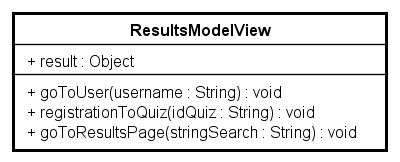
\includegraphics[scale=0.8,keepaspectratio]{UML/Classi/Front-End/QuizziPedia_Front-end_ModelView_ResultsModelView.png}
		\caption{QuizziPedia::Front-End::ModelViews::ResultsModelView}
	\end{figure} \FloatBarrier
	
	\begin{itemize}
		\item \textbf{Descrizione}: classe di tipo modelview la cui istanziazione è contenuta all'interno della variabile di ambiente \$scope di \textit{Angular.js\ped{G}}. All'interno di essa sono presenti le variabili e i metodi necessari per il \textit{Two-Way Data-Binding\ped{G}} tra la view \texttt{ResultsView} e il controller \texttt{ResultsController};
		\item \textbf{Utilizzo}: viene utilizzata per effettuare il \textit{Two-Way Data-Binding\ped{G}} tra la view \texttt{ResultsView} e il controller \texttt{SearchController} rendendo disponibili variabili e metodi;
		\item \textbf{Relazioni con altre classi}: 
		\begin{itemize}
			\item \textit{OUT} \texttt{ResultsView}: view contenente i risultati della ricerca effettuata, sia gli utenti che i questionari trovati; 
			\item \textit{OUT} \texttt{SearchController}: questa classe permette di gestire la ricerca di questionari e utenti all’interno dell’applicazione;
		\end{itemize}
		\item \textbf{Attributi}: 
		\begin{itemize}
			\item \texttt{+ result: Object} \\ Attributo che contiene i seguenti due campi: 
			\begin{itemize}
				\item \texttt{user: Array[Object]}\\ \texttt{array} contenente un oggetto così formato:\\
				\texttt{+ userDetails: Object} \\ Oggetto contenente i seguenti campi dati:
				\begin{itemize}
					\item \texttt{username}.
				\end{itemize}
				\item \texttt{quiz: Array[Object]}\\ \texttt{array} contenente un oggetto così formato:\\
				\item \texttt{+ questionnaireDetails: Object} \\ Oggetto contenente i seguenti campi dati:
				\begin{itemize}
					\item \texttt{name: String};
					\item \texttt{author: String};
					\item \texttt{topic: String};
					\item \texttt{keywords: Array[String]};
					\item \texttt{idQuiz: ObjectId}.
				\end{itemize}
			\end{itemize}
		\end{itemize}
		\item \textbf{Metodi}: 
		\begin{itemize}
				\item \texttt{+} \texttt{goToUser(username: String): void} \\
				Metodo che gestisce l’evento click sul bottone per visualizzare il profilo dell'utente selezionato. Effettua il redirect alla pagina dell'utente.\\
				\textbf{Parametri}:
				\begin{itemize}
					\item \texttt{username: String} \\
					Parametro contenente l'username dell'utente di cui si vuole visualizzare il profilo;
				\end{itemize} 
				\item \texttt{+} \texttt{registrationToQuiz(idQuiz: String): void} \\
				Metodo che gestisce l’evento click sul pulsante di registrazione al questionario.\\
				\textbf{Parametri}:
				\begin{itemize}
					\item \texttt{idQuiz: String} \\
					Parametro contenente l'id del questionario di cui si vuole effettuare l'iscrizione;
				\end{itemize} 
				\item \texttt{+} \texttt{goToResultsPage(stringSearch: String): void} \\
				Metodo che gestisce l’evento click sul pulsante per effettuare una ricerca.\\
				\textbf{Parametri}:
				\begin{itemize}
					\item \texttt{stringSearch: String} \\
					Parametro contenente la stringa della quale effettuare la ricerca;
				\end{itemize} 
		\end{itemize}
	\end{itemize}

	
	\paragraph{QuizziPedia::Front-End::ModelViews::ResultsOfQuizzesModelView}
	
	\label{QuizziPedia::Front-End::ModelViews::ResultsOfQuizzesModelView}
	
	\begin{figure}[ht]
		\centering
		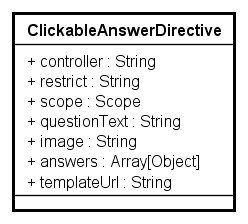
\includegraphics[scale=0.5,keepaspectratio]{UML/Classi/Front-End/QuizziPedia_Front-end_Templates_ClickableAnswerTemplate.png}
		\caption{QuizziPedia::Front-End::ModelViews::HomeModelView}
	\end{figure} \FloatBarrier
	
	\begin{itemize}
		\item \textbf{Descrizione}: classe di tipo modelview la cui istanziazione è contenuta all'interno della variabile di ambiente \$scope di \textit{Angular.js\ped{G}}. All'interno di essa sono presenti le variabili e i metodi necessari per il \textit{Two-Way Data-Binding\ped{G}} tra la view \texttt{ResultsView} e il controller \texttt{ResultsController};
		\item \textbf{Utilizzo}: viene utilizzata per effettuare il \textit{Two-Way Data-Binding\ped{G}} tra la view \texttt{ResultsView} e il controller \texttt{ResultsController} rendendo disponibili variabili e metodi;
		\item \textbf{Relazioni con altre classi}: 
		\begin{itemize}
			\item \textit{IN} \texttt{ResultsView}: view contenente i risultati della ricerca effettuata, sia gli utenti che i questionari trovati; 
			\item \textit{IN} \texttt{ResultsController}: questa classe permette di gestire le iscrizione degli utenti ai questionari;
		\end{itemize}
		\item \textbf{Attributi}: 
		\begin{itemize}
			\item \texttt{+ results: Array} \\ Array contenente un oggetto per ogni iscritto che ha compilato il questionario. L'oggetto sarà composto dai campi: \texttt{nome} e \texttt{cognome} e \texttt{valutazione}.
		\end{itemize}
	\end{itemize}
	
	
	\paragraph{QuizziPedia::Front-End::ModelViews::SignUpModelView}
	
	\label{QuizziPedia::Front-End::ModelViews::SignUpModelView}
	
	\begin{figure}[ht]
		\centering
		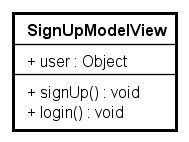
\includegraphics[scale=0.80,keepaspectratio]{UML/Classi/Front-End/QuizziPedia_Front-end_ModelView_SignUpModelView.png}
		\caption{QuizziPedia::Front-End::ModelViews::SignUpModelView}
	\end{figure} \FloatBarrier
	
	\begin{itemize}
		\item \textbf{Descrizione}: classe di tipo modelview la cui istanziazione è contenuta all'interno della variabile di ambiente \$scope di \textit{Angular.js\ped{G}}. All'interno di essa sono presenti le variabili e i metodi necessari per il \textit{Two-Way Data-Binding\ped{G}} tra la view \texttt{SignUpView} e il controller \texttt{SignUpController};
		\item \textbf{Utilizzo}: viene utilizzata per effettuare il \textit{Two-Way Data-Binding\ped{G}} tra la view \texttt{SignUpView} e il controller \texttt{SignUpController} rendendo disponibili variabili e metodi;
		\item \textbf{Relazioni con altre classi}: 
		\begin{itemize}
			\item \textit{OUT} \texttt{SignUpView}: view contenente le form dedicate alla registrazione utente. Contiene inoltre un link alla pagina di login; 
			\item \textit{OUT} \texttt{SignUpController}: questa classe permette di gestire la registrazione di un utente al sistema;
		\end{itemize}
		\item \textbf{Attributi}: 
		\begin{itemize}
			\item \texttt{+ user: Object} \\ Campo dati contenente i seguenti attributi: \texttt{name: String}, \texttt{surname: String}, \texttt{username: String}, \texttt{email: String}, \texttt{password: String} e \texttt{passwordCheck: String};
		\end{itemize}
		\item \textbf{Metodi}: 
		\begin{itemize}
			\item \texttt{+} \texttt{signUp(): void} \\
			Metodo che richiama il metodo \texttt{signUp} del service \texttt{AuthService} passandogli un oggetto di tipo \texttt{SignUpModelView}. Nel caso di buona riuscita dell'operazione viene mostrato un messaggio di successo. Con l'azione di click sul bottone presentato dal messaggio di successo è possibile effettuare il redirect alla pagina di login dell'applicazione. Nel caso in cui invece avvenga un errore, viene mostrato a video il messaggio di errore;
			\item \texttt{+} \texttt{logIn(): void} \\
			Metodo che gestisce l’evento click sul pulsante di login. Effettua il redirect alla pagina di login;
		\end{itemize}
	\end{itemize}
	
	
	\paragraph{QuizziPedia::Front-End::ModelViews::StatisticsModelView}

\label{QuizziPedia::Front-End::ModelViews::StatisticsModelView}

\begin{figure}[ht]
	\centering
	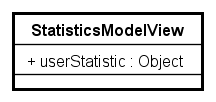
\includegraphics[scale=0.5,keepaspectratio]{UML/Classi/Front-End/QuizziPedia_Front-end_ModelView_StatisticsModelView.png}
	\caption{QuizziPedia::Front-End::ModelViews::StatisticsModelView}
\end{figure} \FloatBarrier

\begin{itemize}
	\item \textbf{Descrizione}: classe di tipo modelview la cui istanziazione è contenuta all'interno della variabile di ambiente \$scope di \textit{Angular.js\ped{G}}. All'interno di essa sono presenti le variabili e i metodi necessari per il \textit{Two-Way Data-Binding\ped{G}} tra la view \texttt{UserView} e il controller \texttt{StatisticsController};
	\item \textbf{Utilizzo}: viene utilizzata per effettuare il \textit{Two-Way Data-Binding\ped{G}} tra la view \texttt{UserView} e il controller \texttt{StatisticsController} rendendo disponibili variabili e metodi;
	\item \textbf{Relazioni con altre classi}: 
	\begin{itemize}
		\item \textit{OUT} \texttt{UserView}: view contenente le direttive dei dati personali dell'utente, delle sue statistiche relative ai questionari e agli allenamenti effettuati e dei questionari a cui è iscritto; 
		\item \textit{OUT} \texttt{StatisticsController}: questa classe permette di le statistiche di un utente.
	\end{itemize}
	\item \textbf{Attributi}: 
	\begin{itemize}
		\item \texttt{+ userStatistic: Object} \\ Oggetto contenente le statistiche di un utente.
	\end{itemize}
\end{itemize}	


	\paragraph[QuizziPedia::Front-End::ModelViews\\::StringsSortingQuestionsModelView]{QuizziPedia::Front-End::ModelViews::StringsSortingQuestionsModelView}
\begin{figure} [ht]
	\centering
	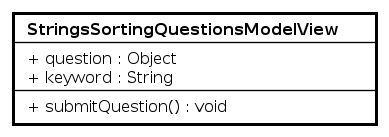
\includegraphics[scale=0.80]{UML/Classi/Front-End/QuizziPedia_Front-end_ModelView_StringsSortingQuestionsModelView.png}
	\caption{QuizziPedia::Front-End::ModelViews::StringsSortingQuestionsModelView}
\end{figure} \FloatBarrier
\begin{itemize}
	\item \textbf{Descrizione}: classe di tipo modelview la cui istanziazione è contenuta all'interno della variabile di ambiente \texttt{\$scope} di \textit{Angular\ped{G}}. All'interno di essa sono presenti le variabili e i metodi necessari per il \textit{Two-Way Data-Binding\ped{G}} tra la \textit{view\ped{G}} \texttt{StringsSortingQuestionsView} e il \textit{controller\ped{G}} \texttt{StringsSortingQuestionsController}; 
	\item \textbf{Utilizzo}: viene utilizzata per effettuare il \textit{Two-Way Data-Binding\ped{G}} tra la \textit{view\ped{G}}\\ \texttt{StringsSortingQuestionsView} e il \textit{controller\ped{G}} \texttt{StringsSortingQuestionsController} rendendo disponibili variabili e metodi;
	\item \textbf{Relazioni con altre classi}:
	\begin{itemize}
		\item \textbf{IN \texttt{StringsSortingQuestionsView}}: \textit{view\ped{G}} contenente i campi e le direttive per creare una domanda a ordinamento stringhe; 
		\item \textbf{IN \texttt{StringsSortingQuestionsController}}: questa classe permette di gestire la creazione e la modifica di una domanda a ordinamento di stringhe.
	\end{itemize}
	\item \textbf{Attributi}:
	\begin{itemize}
			\item \texttt{+ question: Object} \\ Oggetto contenente gli attributi per la creazione della domanda:
			\begin{itemize}
				\item \texttt{answer}: \texttt{array} contenente oggetti che rappresentano le risposte. Ogni oggetto risposta contiene:
				\begin{enumerate}
					\item \texttt{textSorting}: attributo di tipo \texttt{String} che contiene il testo della risposta;
					\item \texttt{position}: attributo di tipo \texttt{Number} che indica la giusta posizione del testo.
				\end{enumerate}
			\end{itemize}
			\item \texttt{+ keyword: String} \\ Attributo contenente la keyword associata alla domanda/questionario.  
	\end{itemize}
	\item \textbf{Metodi}:
	\begin{itemize}
		\item \texttt{+ submitQuestion(): void}\\ 
		Metodo che gestisce l’evento click sul pulsante di conferma sulla domanda. Raccoglie i dati dal modelview e li manda al server attraverso \texttt{QuestionService}. Poi verrà effettuato il redirect alla pagina di gestione delle domande oppure al questionario che si stava creando.
	\end{itemize}
\end{itemize}


		\paragraph{QuizziPedia::Front-End::ModelViews::TrainingModelView}
	
	\label{QuizziPedia::Front-End::ModelViews::TrainingModelView}
	
	\begin{figure}[ht]
		\centering
		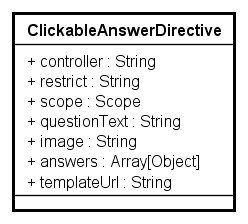
\includegraphics[scale=0.5,keepaspectratio]{UML/Classi/Front-End/QuizziPedia_Front-end_Templates_ClickableAnswerTemplate.png}
		\caption{QuizziPedia::Front-End::ModelViews::LoginModelView}
	\end{figure} \FloatBarrier
	
	\begin{itemize}
		\item \textbf{Descrizione}: classe di tipo modelview la cui istanziazione è contenuta all'interno della variabile di ambiente \$scope di \textit{Angular.js\ped{G}}. All'interno di essa sono presenti le variabili e i metodi necessari per il \textit{Two-Way Data-Binding\ped{G}} tra la view \texttt{TrainingView} e il controller \texttt{TrainingController};
		\item \textbf{Utilizzo}: viene utilizzata per effettuare il \textit{Two-Way Data-Binding\ped{G}} tra la view \texttt{TrainingView} e il controller \texttt{TrainingController} rendendo disponibili variabili e metodi;
		\item \textbf{Relazioni con altre classi}: 
		\begin{itemize}
			\item \textit{OUT} \texttt{TrainingView}: view principale della modalità allenamento, conterrà i vari templates di ogni domanda dell'allenamento; 
			\item \textit{OUT} \texttt{TrainingController}: questa classe permette di gestire la modalità allenamento sottoponendo all'utente le giuste domande adatte al suo livello.
		\end{itemize}
		\item \textbf{Attributi}: 
		\begin{itemize}
			\item \texttt{+ training: Object} \\ Oggetto contenente al suo interno i seguenti campi:
			\begin{itemize}
				\item \texttt{+ argument: String} \\ Attributo contenente l'argomento scelto dall'utente per l'allenamento;
				\item \texttt{+ keywords: Array[String]} \\ Attributo contenente l'\texttt{array} di keywords scelte dall'utente per l'allenamento;
				\item \texttt{+ questionNumber: String} \\ Attributo che rappresenta il numero progressivo della domanda attuale;
				\item \texttt{+ numberOfQuestions: String} \\ Attributo che rappresenta il numero di domande scelte.
			\end{itemize}
		\end{itemize}
		\item \textbf{Metodi}: 
		\begin{itemize}
			\item \texttt{+} \texttt{addQuestion(question: QuestionItemModel): void} \\
			Metodo che gestisce l'evento per inserire una domanda nella cronologia delle domande. \\
			\textbf{Parametri}:
			\begin{itemize}
				\item \texttt{question: QuestionItemModel} \\
				Parametro contenente un riferimento all'oggetto di tipo \texttt{QuestionItemModel};
			\end{itemize}
			\item \texttt{+} \texttt{loadNewQuestionBy(topic: String, keywords: Array[String], level: Number): void} \\
			Metodo che emette l'evento per scaricare una nuova domanda in base ai parametri passati. \\
			\textbf{Parametri}:
			\begin{itemize}
				\item \texttt{topic: String} \\
				Parametro contenente l'argomento della domanda;
				\item \texttt{keywords: Array[String]} \\
				Parametro contenente un\texttt{array} di stringhe che rappresenta le keywords scelte per l'allenamento;
				\item \texttt{level: Number} \\
				Parametro contenente il livello dell'utente.
			\end{itemize}
			\item \texttt{+} \texttt{addResult(questionNumber: Number, result: Boolean): void} \\
			Metodo che gestisce l'evento per inserire il risultato di una domanda nella cronologia delle domande. \\
			\textbf{Parametri}:
			\begin{itemize}
				\item \texttt{questionNumber: Number} \\
				Parametro contenente il numero della domanda risposta;
				\item \texttt{result: Boolean} \\
				Parametro contenente il risultato della domanda risposta.
			\end{itemize}
			\item \texttt{+} \texttt{startTraining(numberOfQuestions: Number, topic: String, keywords: Array[String]): void} \\
			Metodo che gestisce l'evento per iniziare l'allenamento. \\
			\textbf{Parametri}:
			\begin{itemize}
				\item \texttt{numberOfQuestions: Number} \\
				Parametro contenente il numero di domande per l'allenamento;
				\item \texttt{topic: String} \\
				Parametro contenente l'agomento dell'allenamento;
				\item \texttt{keywords: Array[String]} \\
				Parametro contenente \texttt{array} di parole chiave.
			\end{itemize}
		\end{itemize}
	\end{itemize}
	
	
	\paragraph{QuizziPedia::Front-End::ModelViews::TrueFalseQuestionsModelView}
\begin{figure} [ht]
	\centering
	%\includegraphics[scale=0.80]{UML/Classi/Front-End/QuizziPedia_Front-end_Views_TrueFalseQuestionsModelView.png}
	\caption{QuizziPedia::Front-End::ModelViews::TrueFalseQuestionsModelView}
\end{figure} \FloatBarrier
\begin{itemize}
	\item \textbf{Descrizione}: classe di tipo modelview la cui istanziazione è contenuta all'interno della variabile di ambiente \$scope di \textit{Angular.js\ped{G}}. All'interno di essa sono presenti le variabili e i metodi necessari per il \textit{Two-Way Data-Binding\ped{G}} tra la view \texttt{TrueFalseQuestionsView} e il controller \texttt{TrueFalseQuestionsController}; 
	\item \textbf{Utilizzo}: viene utilizzata per effettuare il \textit{Two-Way Data-Binding\ped{G}} tra la view \texttt{TrueFalseQuestionsView} e il controller \texttt{TrueFalseQuestionsController} rendendo disponibili variabili e metodi;
	\item \textbf{Relazioni con altre classi}:
	\begin{itemize}
		\item \textit{IN} \texttt{TrueFalseQuestionsController}: questa classe permette di gestire la creazione e la modifica di una domanda vero/falso;
		\item \textit{OUT} \texttt{TrueFalseQuestionsView}: view contenente le direttive per creare una domanda vero/falso.
	\end{itemize}
	\item \textbf{Attributi}:
	\begin{itemize}
	  \item \texttt{question: Object} \\ Oggetto contenete i dati della domanda, ovvero:
	  \begin{itemize}
		\item \texttt{questionText: String}: identifica il testo della domanda;
		\item \texttt{image: String}: identifica l'url di una possibile immagine nella domanda;
		\item \texttt{answers: Array}: array che contiene coppie di valori. Queste coppie sono formate da:
		\begin{itemize}
			\item \texttt{type: String}: indica la tipologia della risposta;
			\item \texttt{text: String}: contiene il testo dell'affermazione;
			\item \texttt{url: String}: rappresenta l'immagine della risposta;
			\item \texttt{attributesForTForMultiple: Mixed}: contiene i seguenti attributi:
			\begin{enumerate}
				\item \texttt{isItRight: Boolean}: contiene se la risposta è vera o falsa.
			\end{enumerate}
		\end{itemize}
	\end{itemize}
	\end{itemize}
	\item \textbf{Metodi}:
	\begin{itemize}
		\item \texttt{+} \texttt{submitQuestion(): void}\\ 
		Metodo che gestisce l’evento click sul pulsante di conferma sulla domanda. Raccoglie i dati dal modelview e li manda al server attraverso \texttt{QuestionService}. Poi verrà effettuato il redirect alla pagina di gestione delle domande oppure al questionario che si stava creando;
	\end{itemize}
\end{itemize}


	\paragraph{QuizziPedia::Front-End::ModelViews::UserDetailsModelView}
		
		\label{QuizziPedia::Front-End::ModelViews::UserDetailsModelView}
		
		\begin{figure}[ht]
			\centering
			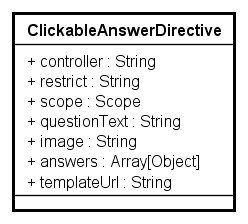
\includegraphics[scale=0.5,keepaspectratio]{UML/Classi/Front-End/QuizziPedia_Front-end_Templates_ClickableAnswerTemplate.png}
			\caption{QuizziPedia::Front-End::ModelViews::UserDetailsModelView}
		\end{figure} \FloatBarrier
		
		\begin{itemize}
			\item \textbf{Descrizione}: classe di tipo modelview la cui istanziazione è contenuta all'interno della variabile di ambiente \$scope di \textit{Angular.js\ped{G}}. All'interno di essa sono presenti le variabili e i metodi necessari per il \textit{Two-Way Data-Binding\ped{G}} tra la view \texttt{UserView} e il controller \texttt{UserDetailsController};
			\item \textbf{Utilizzo}: viene utilizzata per effettuare il \textit{Two-Way Data-Binding\ped{G}} tra la view \texttt{UserView} e il controller \texttt{UserDetailsController} rendendo disponibili variabili e metodi;
			\item \textbf{Relazioni con altre classi}: 
			\begin{itemize}
				\item \textit{IN} \texttt{UserView}: view contenente le direttive dei dati personali dell'utente, delle sue statistiche relative ai questionari e agli allenamenti effettuati e dei questionari a cui è iscritto; 
				\item \textit{IN} \texttt{UserDetailsController}: questa classe permette di ottenere i dati di un utente;
			\end{itemize}
			\item \textbf{Attributi}: 
			\begin{itemize}
				\item \texttt{+ username: String} \\ Attributo che conterrà l'username dell'utente ricercato.
			\end{itemize}
		\end{itemize}
		
			